En este capítulo se explicará el funcionamiento de la aplicación desde el punto
de vista del usuario final, detallando las opciones de cada una de las secciones.

Para poder acceder a la aplicación, tal y como se explicó en el apéndice 
\textit{\nameref{sec:maninstalacion}}, será necesario utilizar el comando:

\begin{minted}{bash}
  ./oflute
\end{minted}

\section{Ejecución inicial}
Al lanzar la aplicación, se abrirá una ventana y aparecerán, consecutivamente,
la pantalla de créditos del autor y la pantalla de presentación del
juego. Pasados unos momentos éstas desaparecerán, aunque tiene la opción de
omitir cada una de las pantallas pulsando la tecla \texttt{escape}.

\begin{figure}[h!]
  \centering
  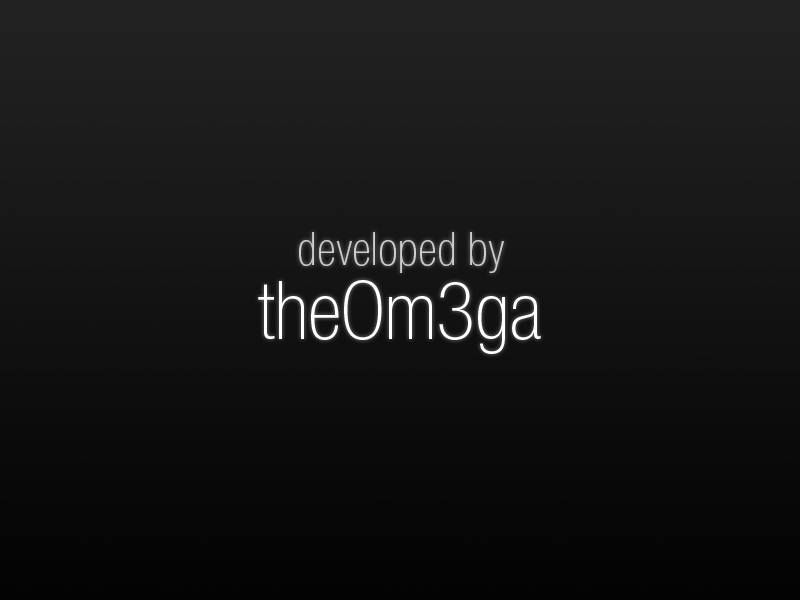
\includegraphics[width=0.8\textwidth]{apendice_manual_usuario/imagen_estadoAutor}
  \caption{Pantalla de créditos del autor}
  \vspace{-1cm}
\end{figure}

\begin{figure}[h!]
  \centering
  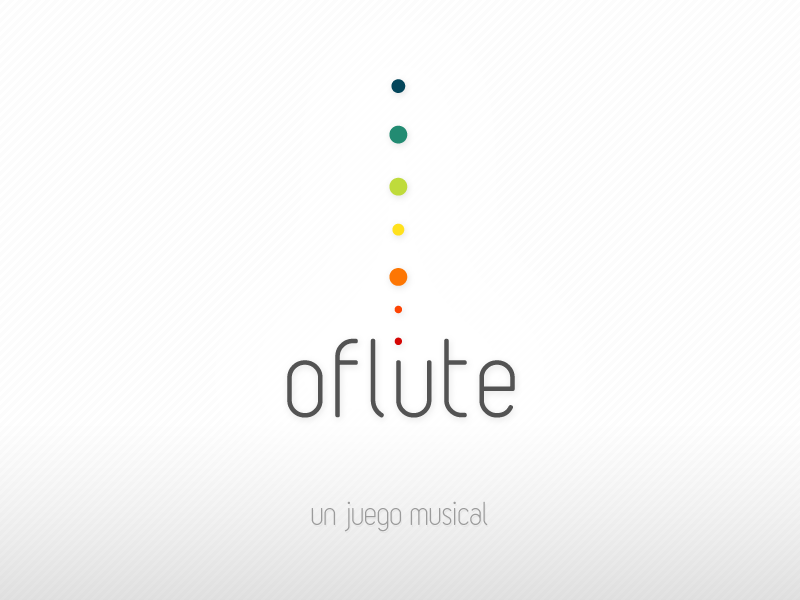
\includegraphics[width=0.8\textwidth]{apendice_manual_usuario/imagen_estadoIntro}
  \caption{Pantalla de presentación del juego}
  \vspace{-0.3cm}
\end{figure}

Una vez desaparezcan ambas pantallas, se iniciará una animación para mostrar el
menú principal. Puede cancelar la animación y mostrar rápidamente el menú
principal pulsando la tecla \texttt{escape}.

\begin{figure}[h!]
  \vspace{-0.1cm}
  \centering
  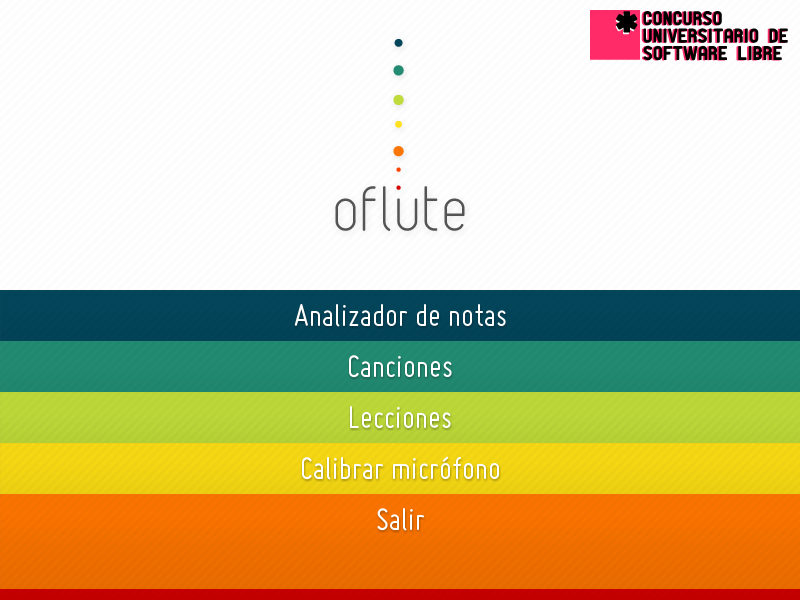
\includegraphics[width=0.8\textwidth]{apendice_manual_usuario/imagen_menuPrincipal}
  \caption{Pantalla del menú principal}
  \vspace{-1cm}
\end{figure}

Cuando las animaciones concluyan, el menú principal ya será completamente
funcional. Podremos acceder a las diferentes opciones, ya sea haciendo click con
el ratón en los botones de pantalla, o pulsando alguna de las teclas de acceso
directo. Las secciones y teclas asignadas son las siguientes:

\begin{itemize}
\item \textbf{Analizador de notas} (\textit{tecla 1}) Abre el analizador de
  notas.
\item \textbf{Canciones} (\textit{tecla 2}) Pasa al menú de selección de
  canciones.
\item \textbf{Lecciones} (\textit{tecla 3}) Abre el menú de elección de
  lecciones.
\item \textbf{Calibrar micrófono} (\textit{tecla 4}) Lanza el sistema de
  calibración del micrófono.
\item \textbf{Salir} (\textit{tecla 5}) Cierra la aplicación
\end{itemize}

Lo recomendado, en la primera ejecución de \textbf{oFlute}, es lanzar la sección
\textit{Calibrar micrófono}, ya sea pulsando el botón con el ratón o mediante la
tecla 4. Con esto nos cercioramos de que el programa es capaz de distinguir el
sonido del micrófono del ruido de fondo. Una vez hecho, ya estará todo listo
para acceder al resto de secciones.

\section{Sección -- calibrar micrófono}
Pulsando el botón correspondiente, o mediante la tecla 4, pasaremos a la sección
de calibración del micrófono. En primer lugar, aparecerá el siguiente mensaje:

\begin{figure}[h!]
  \vspace{-0.1cm}
  \centering
  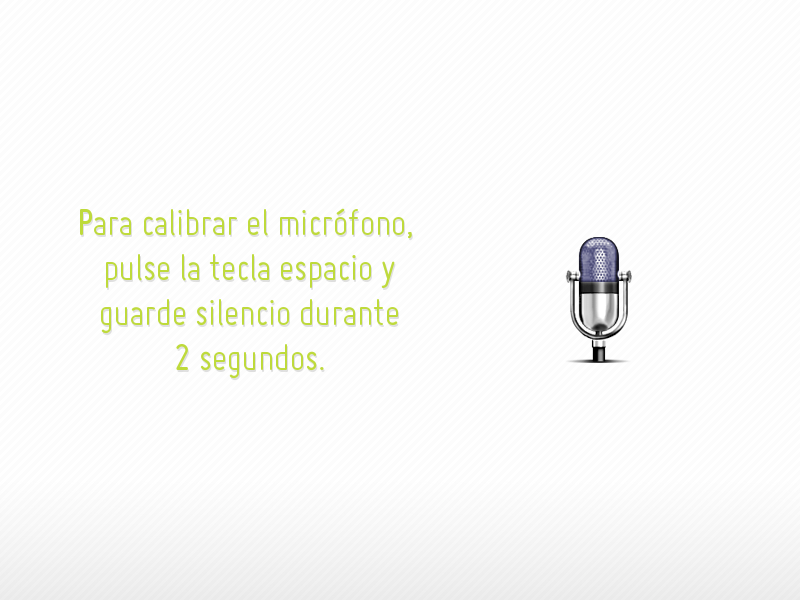
\includegraphics[width=0.8\textwidth]{apendice_manual_usuario/imagen_seccionCalibrar1}
  \caption{Pantalla inicial de calibración del micrófono}
  \vspace{-1cm}
\end{figure}

Como se indica en el mensaje, para comenzar la calilbración el usuario deberá
pulsar la tecla \texttt{espacio} y guardar silencio en el micrófono durante dos
segundos. En ese momento, aparecerá el siguiente mensaje:

\begin{figure}[h!]
  \vspace{-0.1cm}
  \centering
  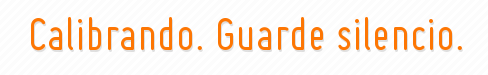
\includegraphics[width=0.8\textwidth]{apendice_manual_usuario/imagen_seccionCalibrar_mensaje1}
  \caption{Mensaje al inicio del calibrado}
\end{figure}

Una vez pasen los dos segundos y concluya la calibración, se mostrará el
siguiente mensaje:

\begin{figure}[h!]
  \vspace{-0.1cm}
  \centering
  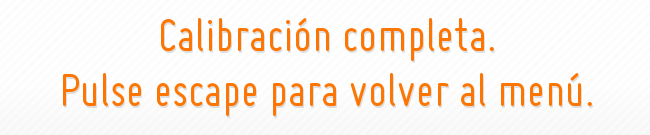
\includegraphics[width=0.8\textwidth]{apendice_manual_usuario/imagen_seccionCalibrar_mensaje2}
  \caption{Mensaje al final del calibrado}
\end{figure}

Cuando concluya el proceso, la aplicación habrá guardado el valor umbral de
ruido del micrófono, lo que facilitará el análisis del sonido de la flauta.

Hay casos en los que la calibración será defectuosa, y un mensaje informará de
ello. En tal caso, no habrá más que comprobar la configuración del micrófono y
repetir el proceso de calibrado.

\section{Sección -- analizador de notas}

Al pulsar el botón correspondiente a la sección del analizador de notas,
mediante una animación aparecerán los elementos de esta parte de la aplicación
(figura \ref{fig:pantalla_analizador_notas} en página
\pageref{fig:pantalla_analizador_notas}).

\begin{figure}[h!]
  \vspace{-0.1cm}
  \centering
  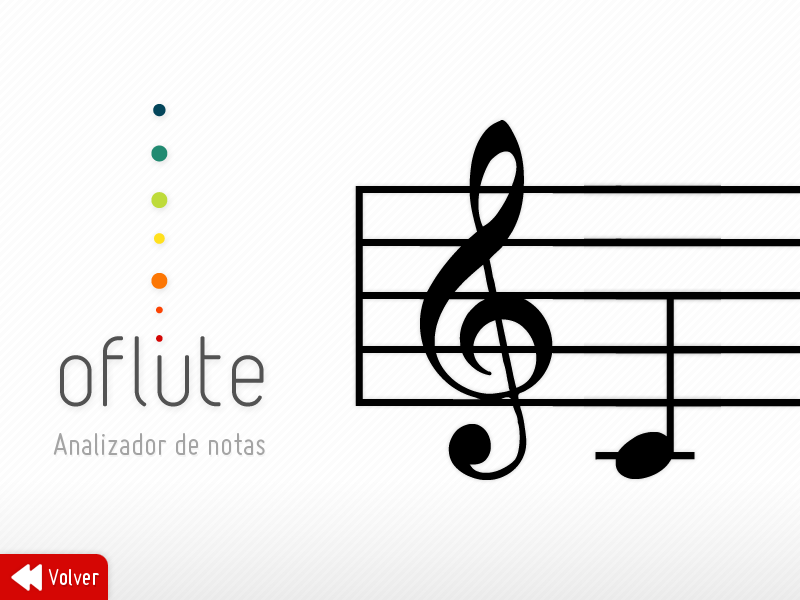
\includegraphics[width=0.75\textwidth]{apendice_manual_usuario/imagen_seccionAnalizador}
  \caption{Pantalla del analizador de notas}
  \label{fig:pantalla_analizador_notas}
\end{figure}

Una vez terminen de mostrarse todos los elementos, el usuario podrá empezar a
utilizar la funcionalidad de la sección. En concreto, el analizador de notas nos
permite ver reflejada en el pentagrama la nota que toquemos con la flauta.

Su uso, pues, es muy sencillo. Simplemente tendremos que tocar nuestra flauta de
forma que el micrófono sea capaz de captar su sonido. Si lo hacemos
correctamente, el analizador mostrará en cada momento la nota que está tocando
sobre el pentagrama.

Una vez hayamos acabado de utilizar esta sección de la aplicación, podremos
pulsar en el botón \textit{Volver}, o en la tecla \texttt{escape} del teclado,
lo que nos llevará de vuelta al menú principal.

\section{Sección -- lecciones}
\vspace{-0.5cm}
Si seleccionamos la opción \textit{Lecciones} en el menú principal, o
alternativamente presionamos la tecla 3 del teclado, la aplicación mostrará una
animación para ocultar el menú principal y nos mostrará el menú de selección de
lecciones. 

\begin{figure}[h!]
  \vspace{-0.2cm}
  \centering
  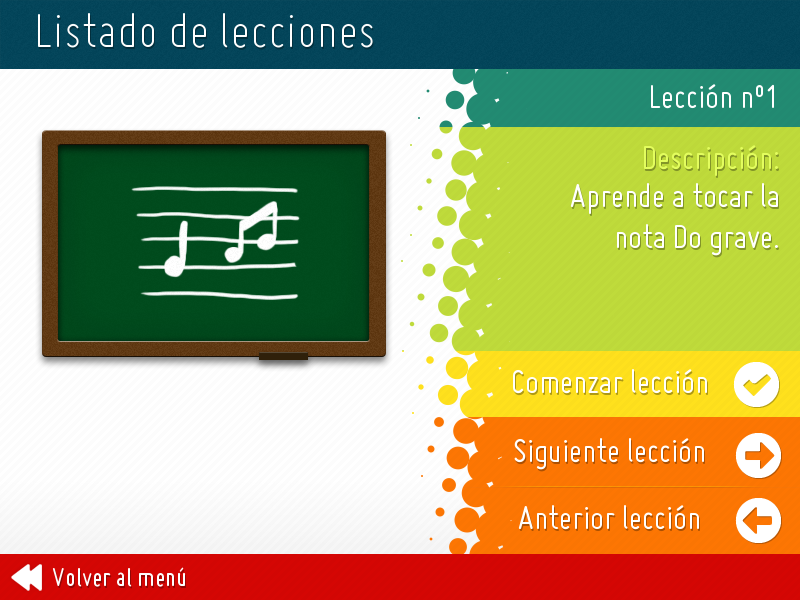
\includegraphics[width=0.75\textwidth]{apendice_manual_usuario/imagen_seccionLecciones1}
  \caption{Pantalla del menú de selección de lecciones}
  \vspace{-1cm}
\end{figure}

\pagebreak

En cualquier momento podemos hacer click en el botón \textit{Volver al menú}, o
pulsar la tecla \texttt{escape} del teclado, para ir a la sección anterior.

En el menú de selección de lecciones podremos encontrar los siguientes
elementos:

\begin{itemize}
\item \textbf{Título} de la lección
\item \textbf{Descripción} de la lección
\item Botón \textbf{Comenzar lección}.
\item Botón \textbf{Anterior lección}.
\item Botón \textbf{Siguiente lección}.
\item Botón \textbf{Volver al menú}.
\end{itemize}

Mediante los botones de \textit{anterior} y \textit{siguiente lección} podremos
navegar entre las diferentes lecciones cargadas en el sistema. Haciendo uso de
los paneles de \textit{título} y \textit{descripción} nos informaremos sobre la
lección elegida. Una vez que tengamos claro la lección que queremos tomar,
pulsaremos en el botón \textit{comenzar lección.}

Una vez que decidamos comenzar la lección, el sistema ocultará los elementos del
menú de selección de lecciones mediante animaciones y, posteriormente, cargará y
mostrará los elementos de la lección elegida.

\begin{figure}[h!]
  \centering
  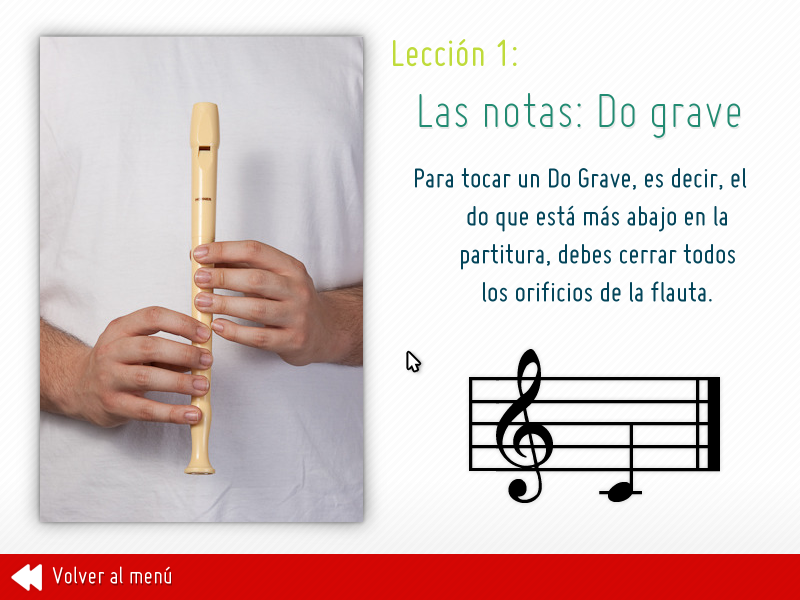
\includegraphics[width=0.8\textwidth]{apendice_manual_usuario/imagen_seccionLecciones2}
  \caption{Pantalla de lección de ejemplo}
\end{figure}

Las lecciones se muestran en forma de conjunto de elementos multimedia --
imágenes y texto -- de fácil comprensión, que el usuario podrá leer y estudiar
de forma independiente. En futuras versiones de la aplicación se podrán utilizar
lecciones de varias etapas, así como integrar sonidos y otro tipo de multimedia.

\section{Sección -- canciones}

El usuario podrá acceder a esta sección desde el menú principal, pulsando en la
botón \textit{Canciones}, o con la tecla 2 del teclado.

Al acceder, desaparecerá el menú principal y se mostrará el menú de selección de
canciones.

\begin{figure}[h!]
  \centering
  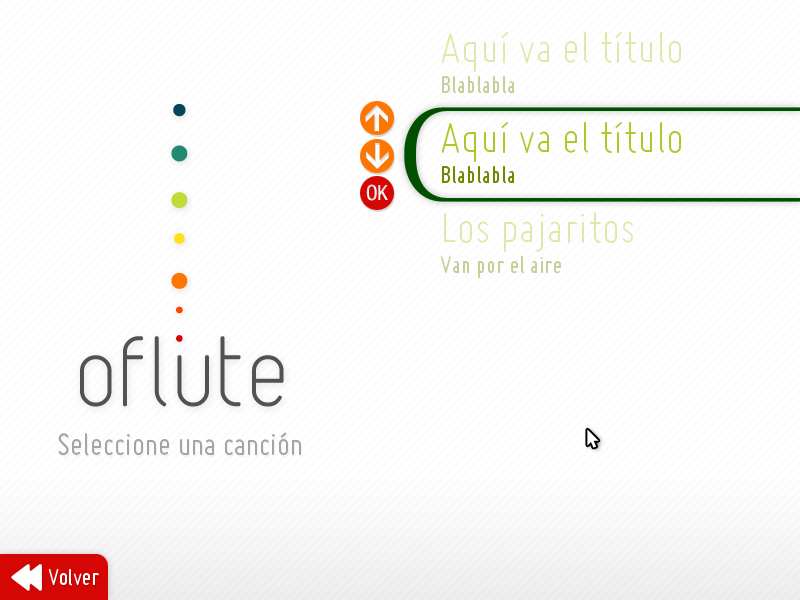
\includegraphics[width=0.8\textwidth]{apendice_manual_usuario/imagen_seccionCanciones1}
  \caption{Pantalla del menú de selección de canciones}
\end{figure}

Esta pantalla consta de los siguientes botones:
\begin{itemize}
\item \textbf{Anterior canción}, representado con una flecha hacia arriba.
\item \textbf{Siguiente canción}, representado con una flecha hacia abajo.
\item \textbf{Comenzar canción}, simbolizado con la palabra \textit{OK}.
\item \textbf{Volver}.
\end{itemize}

Mediante los botones \textit{anterior} y \textit{siguiente canción}, el usuario
podrá elegir el tema a interpretar con la flauta. Una vez esté resaltada la
canción correcta, el usuario deberá pulsar el botón \textit{Comenzar canción --
  OK} para que dé comienzo la interpretación.

También es posible pulsar el botón \textit{volver} para ir de nuevo al menú
principal.

\subsection{Interpretación de la canción}

Al lanzar la canción, aparecerá la pantalla de interpretación de canción, que
contiene numerosos elementos importantes para el jugador.

\begin{figure}[h!]
  \centering
  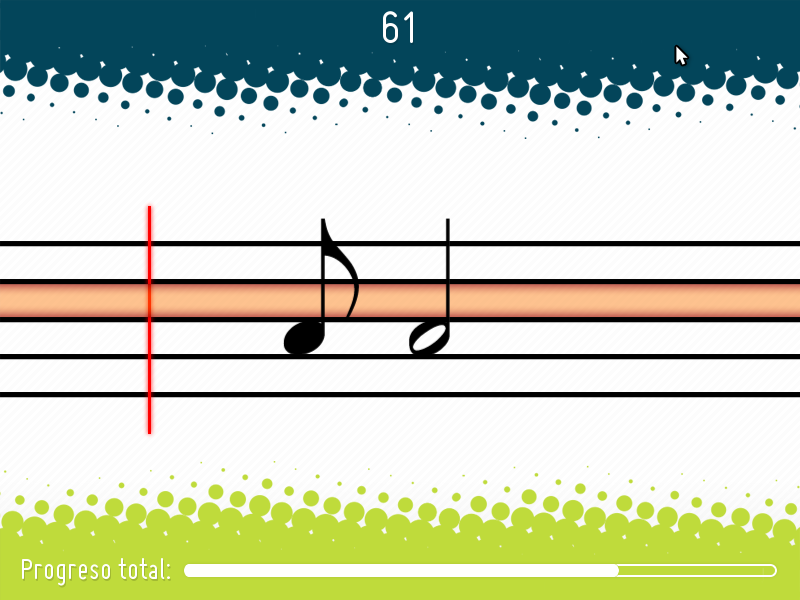
\includegraphics[width=0.8\textwidth]{apendice_manual_usuario/imagen_seccionCanciones2}
  \caption{Pantalla de interpretación de canción}
\end{figure}

\begin{enumerate}
\item \textbf{Marcador} de la puntuación del usuario.
\item \textbf{Pentagrama}. Sobre él aparecerán las notas.
\item \textbf{Notas}. Éstas irán apareciendo por el lado derecho del pentagrama,
  y moviéndose hacia la izquierda de forma ordenada y rítmica.
\item \textbf{Resaltado de nota}. Resalta la posición en el pentagrama de la
  nota que está tocando el usuario con la flauta en cada momento. Esto ayuda
  visualmente a saber si estamos interpretando la nota correcta o no.
\item \textbf{Barra de interpretación}. Esta barra indica cuándo debe el usuario
  empezar a tocar la nota. 
\item \textbf{Barra de progreso}. Indica el progreso de la interpretación de la
  canción. Cuando la barra esté completa, la canción concluirá.
\end{enumerate}

La forma de juego es sencilla. Como se ha indicado, las notas aparecerán sobre
el pentagrama por el lado derecho, e irán desplazándose hacia la izquierda. Una
vez que una nota llegue a la \textit{barra de interpretación}, el jugador deberá
tocar con la flauta la nota correcta, de forma constante hasta que llegue el
turno de la siguiente nota.

Para ayudar al jugador, la barra de \textit{resaltado de nota} indicará en cada
momento qué nota se está tocandoo. Así, si en un instante es necesario tocar un
\textit{Sol} pero la barra de resaltado está por encima, el usuario sabrá que
debe cerrar más orificios de la flauta.

Las posibles \textbf{notas} que pueden aparecer son \textit{Do}, \textit{Re},
\textit{Mi}, \textit{Fa}, \textit{Sol}, \textit{La}, \textit{Si}, \textit{Do
  grave} y \textit{Re grave}. Las posibles figuras que podrán aparecer son las
siguientes:

\begin{description}
\item[Redonda] -- Dura cuatro tiempos.
\vspace{-0.1cm}
\begin{figure}[h!]
  \centering
  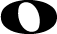
\includegraphics[width=0.05\textwidth]{apendice_manual_usuario/imagen_figRedonda}
  \caption{Figura musical -- Redonda}
\end{figure}

\vspace{-0.35cm}

\item[Blanca] -- Dura dos tiempos.
\vspace{-0.1cm}
\begin{figure}[h!]
  \centering
  \subfloat[Posición normal]{\parbox{0.5\textwidth}{\centering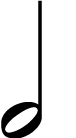
\includegraphics[width=1cm]{apendice_manual_usuario/imagen_figBlanca}}}
  \subfloat[Posición invertida]{\parbox{0.5\textwidth}{\centering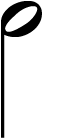
\includegraphics[width=1cm]{apendice_manual_usuario/imagen_figBlancaInv}}}
  \caption{Figura musical -- Blanca}
\end{figure}

\vspace{-0.35cm}

\item[Negra] -- Dura un tiempo.
\vspace{-0.1cm}
\begin{figure}[h!]
  \centering
  \subfloat[Posición normal]{\parbox{0.5\textwidth}{\centering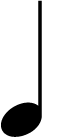
\includegraphics[width=1cm]{apendice_manual_usuario/imagen_figNegra}}}
  \subfloat[Posición invertida]{\parbox{0.5\textwidth}{\centering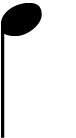
\includegraphics[width=1cm]{apendice_manual_usuario/imagen_figNegraInv}}}
  \caption{Figura musical -- Negra}
\end{figure}

\vspace{-0.35cm}

\item[Corchea] -- Dura la mitad que una negra.
\vspace{-0.1cm}
\begin{figure}[h!]
  \centering
  \subfloat[Posición normal]{\parbox{0.5\textwidth}{\centering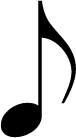
\includegraphics[width=1cm]{apendice_manual_usuario/imagen_figCorchea}}}
  \subfloat[Posición invertida]{\parbox{0.5\textwidth}{\centering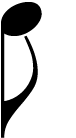
\includegraphics[width=1cm]{apendice_manual_usuario/imagen_figCorcheaInv}}}
  \caption{Figura musical -- Corchea}
\end{figure}
\end{description}

\vspace{-0.35cm}

De manera excepcional, es posible alargar el tiempo de una figura mediante el
uso del \textbf{puntillo}, que hará que su duración aumente la mitad de su
tiempo original. El puntillo se representa mediante un pequeño círculo a la
derecha de la base de la nota.

Por otro lado, las siguientes son las figuras que representan los silencios
